\section{Deep Learning approach}
\label{sec32}

Deep Learning (DL) is a subfield of machine learning.
DL was developed as a solution to the problem of feature engineering extraction, which necessitates a high level of experience and talent to extract damage-sensitive features for specific SHM applications.
DL is a type of representation learning that recognizes the appropriate data representa\-tions for models like classification and detection.

It can be said that DL techniques have progressed rapidly in recent years as a result of significant advancements in computational power (e.g., central processing units (CPU), graphical processing units (GPU), etc.), as well as the availability of big data and the development of new learning algorithms~\cite{Yuan2020}.
As a result, DL-based SHM methods have been used to address difficulties with ML-based SHM.

DL was first motivated by the way the human brain learns.
It has a large number of neurons that are densely connected to build a hierarchical structure capable of receiving data from the visual cortex, which can recognise the distinct shapes of edges of an object.
These learned patterns are then transferred to a brain area capable of detecting more complex patterns.

DL is a type of hierarchical learning~\cite{Ongsulee2018} in which non-linear functions are used to extract data representations from raw input data~\cite{Lecun2015}.
The collected representation data has simple learnable extracted characteristics at the shallowest layers.
As you progress deeper into the stages, those extracted features become increasingly complica\-ted, learnable features.

\subsection{Multilayer Perceptrons}

The simplest DL networks are called multilayer perceptrons (MLP), which are construct\-ed from a group of multiple layers of perceptrons (artificial neurons).
Hence, the term "deep" comes from multiple layers.
A perceptron has several inputs and outputs, which have weighted connections with a nonlinear activation function.
By performing this operation, a non-linearity is injected into the network, which is important for the learning process.
Therefore, if the non-linearity is not considered, no matter how many layers are in the network, it will act like a single-layer neuron. 
Because by just linearly adding these layers, it will produce another linear output.
As a result, a neuron can not update its weights, resulting in no learning.
Artificial neuron structure is presented in Fig.~\ref{fig:artificial Neuron}.
%%%%%%%%%%%%%%%%%%%%%%%%%%%%%%%%%%%%%%%%%%%%%%%%%%%%%%%%%%%%%%%%%%%%%%%%%%%%%%%%
\begin{figure} [!ht]
	\begin{center}
		\centering
		\includegraphics[scale=1]{Figures/Chapter_1/artificial_neuron.png}
	\end{center}
	\caption{Structure of Perceptron.} 
	\label{fig:artificial Neuron}
\end{figure}
%%%%%%%%%%%%%%%%%%%%%%%%%%%%%%%%%%%%%%%%%%%%%%%%%%%%%%%%%%%%%%%%%%%%%%%%%%%%%%%%
There are several non-linear functions used in artificial neural networks, such as the Rectified Linear Unit (Relu), which is commonly used, as shown in Eqn~(\ref{Eq:relu}):
%%%%%%%%%%%%%%%%%%%%%%%%%%%%%%%%%%%%%%%%%%%%%%%%%%%%%%%%%%%%%%%%%%%%%%%%%%%%%%%%
\begin{equation}
	Relu(z) = 
	\begin{cases}
		0,  \text{  if}\ z<0\\
		z,  \text{  otherwise}
	\end{cases},
	\label{Eq:relu}
\end{equation}
%%%%%%%%%%%%%%%%%%%%%%%%%%%%%%%%%%%%%%%%%%%%%%%%%%%%%%%%%%%%%%%%%%%%%%%%%%%%%%%%
Other non-linear functions are the Sigmoid logistic function as shown in Eqn~(\ref{sigmoid}):
\begin{equation}
	\sigma(z) = \frac{1}{1+e^{-z}},
	\label{sigmoid}
\end{equation}
And hyperbolic tangent function tanh as shown in Eqn~(\ref{tanh})~\cite{Lecun2015}:
\begin{equation}
	\tanh(z)=  \frac{e^z-e^{-z}}{e^z+e^{-z}},
	\label{tanh}
\end{equation}
where \(z\) is the summation of adjustable weights \(\{w_0,w_1,\dots,w_n \}\) multiplied by input variables (from previous layer) \(\{x_0,x_1,\dots,x_n\}\) and a bias \(b\) as shown in Eqn~(\ref{z}):
\begin{equation}
	z= \sum_{i=0}^{n}  w_i\times x_i +b,
	\label{z}
\end{equation}
%%%%%%%%%%%%%%%%%%%%%%%%%%%%%%%%%%%%%%%%%%%%%%%%%%%%%%%%%%%%%%%%%%%%%%%%%%%%%%%%

Supervised learning is the traditional approach to learning in which a neural network builds its knowledge from a given labelled dataset, where the ground truth output is known previously~\cite{Lecun2015}.

\subsubsection{Optimization and Deep Learning}
MLP models learn to find the desired output by updating the network parameters such as weights and biases.
Accordingly, a model does a comparison between the calculated output (predicted) and the ground truth output (target).
For this purpose, an objective function (cost function) is applied to estimate the loss (error) between the predicted output and the target.
Accordingly, this process needs to be optimized to minimize the estimated value of the loss.
A well-known optimization algorithm utilised in DL is the gradient descent (GD)~\cite{Lecun2015}.
Fig.~\ref{fig:GD} illustrates the concept of GD in one dimension, in which weights \(\{w_0,w_1,\dots,w_n\}\) are initially assigned randomly.
GD aims to reduce the cost function \(J(w)\) at each step to reach the \(J_{min}(w)\) (global minimum) by calculating the gradient, which represents the slope of the cost function.
%%%%%%%%%%%%%%%%%%%%%%%%%%%%%%%%%%%%%%%%%%%%%%%%%%%%%%%%%%%%%%%%%%%%%%%%%%%%%%%%
\begin{figure}[!ht]
	\begin{center}
		\centering
		\includegraphics[scale=1]{Figures/Chapter_3/Gradient_decent.png}
	\end{center}
	\caption{The process of Gradient Descent.} 
	\label{fig:GD}
\end{figure}
%%%%%%%%%%%%%%%%%%%%%%%%%%%%%%%%%%%%%%%%%%%%%%%%%%%%%%%%%%%%%%%%%%%%%%%%%%%%%%%%
Accordingly, the weights are modified as shown in Eqn.~(\ref{weight_updates}):
\begin{equation}
	w_{i+1}= w_{i} -\alpha \frac{\partial J(w)}{\partial w_i}, 
	\label{weight_updates}
\end{equation}
where the partial derivative \(\frac{\partial J(w)}{\partial w_i}\) is the gradient, and \(\alpha \) is the learning rate, which is the amount that the weights are updated during the learning process~\cite{Russell2010}.
Therefore, the learning rate monitors the rate at which the neural network learns.
Hence, small learning rates require more training time because of the small changes made to the weights when updated, whereas large learning rates result in accelerated changes, consequently, require less training time:
%%%%%%%%%%%%%%%%%%%%%%%%%%%%%%%%%%%%%%%%%%%%%%%%%%%%%%%%%%%%%%%%%%%%%%%%%%%%%%%%

The backpropagation algorithm is the most widely used learning algorithm for neural networks, in which it back propagates the calculated gradients across all the perceptrons.
Accordingly, all weights and biases are updated, which leads to minimizing the loss value.
\subsubsection{Optimization Challenges in Deep Learning}
The optimization algorithm in DL aims to reach the global minimum value of the cost function \(J(w)\).
However, some challenges during the training process may occur.
The most tricky challenges are the local minima, saddle points, vanishing gradients, and exploding gradients.

The local minima occur during training when the optimization algorithm ends up with a value of the cost function \(J(w)\) that is smaller than values of \(J(w)\) at any other points in the local neighborhood of \(w\).
Figure~\ref{fig:local_minima} shows that during the optimization process, it is possible to end up in local minima.
%%%%%%%%%%%%%%%%%%%%%%%%%%%%%%%%%%%%%%%%%%%%%%%%%%%%%%%%%%%%%%%%%%%%%%%%%%%%%%%%
\begin{figure}[!ht]
	\begin{center}
		\centering
		\includegraphics[scale=1]{Figures/Chapter_3/local_minima.png}
	\end{center}
	\caption{Local minima.} 
	\label{fig:local_minima}
\end{figure}
%%%%%%%%%%%%%%%%%%%%%%%%%%%%%%%%%%%%%%%%%%%%%%%%%%%%%%%%%%%%%%%%%%%%%%%%%%%%%%%%

A saddle point is any location where all gradients of a cost function vanish but is neither a global nor a local minimum, as shown in Fig.~\ref{fig:saddle_point}.

The vanishing gradients are the most encountered problem during the optimization process, as the gradients become too small, causing the learning process to get stuck for a long time before it makes any progress or stops at all~\cite{Brownlee2017a}.
On the other hand, the exploding gradients problem occurs when the gradients become so large that they lead to numerical overflow and result in \enquote{NaN} values~\cite{Brownlee2017a}.
%%%%%%%%%%%%%%%%%%%%%%%%%%%%%%%%%%%%%%%%%%%%%%%%%%%%%%%%%%%%%%%%%%%%%%%%%%%%%%%%
\begin{figure}[!ht]
	\begin{center}
		\centering
		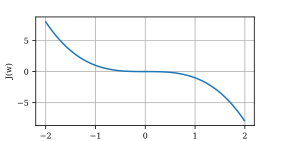
\includegraphics[scale=1]{Figures/Chapter_3/saddle_point.png}
	\end{center}
	\caption{Saddle point.} 
	\label{fig:saddle_point}
\end{figure}
%%%%%%%%%%%%%%%%%%%%%%%%%%%%%%%%%%%%%%%%%%%%%%%%%%%%%%%%%%%%%%%%%%%%%%%%%%%%%%%%
\subsection{Convolutional Neural Network} 
Convolutional Neural Network (CNN) is a special type of artificial neural network (ANN) that was initially developed in the 1980s by ~\textcite{Fukushima1980} who was inspired by the discoveries of Hubel and Wiesel regarding the cat's visual cortex.
CNN is one of the most utilised architectures in DL for image processing as they can recognise complex patterns of images by performing convolution operations.

In mathematics, a convolution is an operation performed between any two functions, as for example \(f, g:\mathbb{R}^{d} \to \mathbb{R}\) to produce a third function \((f\ast g)\) depicted in Eqn.~(\ref{eqn:convolution}):
\begin{equation}
	(f\ast g)(x) = \int_{}^{} f(z)g(x-z)dz
	\label{eqn:convolution}
\end{equation}
In which, we measure the overlap between \(f\) and \(g\), as one function is flipped and shifted by \(x\).

In the case of discrete objects defined on the set \(\mathbb{Z}\) of integers, the integral operation turns into a summation of elementwise multiplied components, as depicted in Eqn.~(\ref{eqn:discrete_conv}):
\begin{equation}		
	(f\ast g)(x) = \sum_{a}^{} f(a)g(i-a)
	\label{eqn:discrete_conv}
\end{equation}
For inputs with two dimensions, we have a corresponding sum with indices \((a,b)\) for \(f\) and \((i-a, j-b)\) for \(y\) respectively as depicted in Eqn.~\ref{eqn:2d_conv} that describes a cross correlation operation:
\begin{equation}
	(f\ast g)(i,j) = \sum_{a}^{}\sum_{b}^{}f(a,b)g(i-a,j-b)
	\label{eqn:2d_conv}
\end{equation}
%%%%%%%%%%%%%%%%%%%% from here
The convolution operation for image processing is essentially a cross-correlation opera\-tion, also known as a sliding dot product or sliding inner-product.
CNN was designed to process data as tensors with different dimensions.
For a 1D data tensor, it can represent various data forms, such as signals and sequences, in addition to sentences in various languages in translation problems.
For a 2D data tensor, it can represent an image in grayscale (one channel). Furthermore, by combining three 2D tensors, a coloured 3D image is produced due to the different intensities of the pixels in the (RGB) channels.
A 4D tensor represents volumetric data, such as a sequence of 3D images or a video.

A convolutional layer has a number \( n\) of convolution kernels (filters), in which each kernel has a set of weights of a size \((w_k,h_k,d_k)\).
The kernel slides over an input image of a size \((w,h,d)\) performing a convolution operation (dot product), where \(w\) and \(h\) represent the image width and height, respectively, while \(d\) represents the depth (number of channels).
The outputs of the convolution operation are feature maps that are locally connected to the outputs of the previous layer.
Figure~\ref{fig:convolution_3d} illustrates the convolution operation for a 3D input and the calculated output (feature map) with a new shape of \((h_{n}\times w_{n} \times d_{n})\).
%%%%%%%%%%%%%%%%%%%%%%%%%%%%%%%%%%%%%%%%%%%%%%%%%%%%%%%%%%%%%%%%%%%%%%%%%%%%%%%%
\begin{figure} [!ht]
	\begin{center}
		\centering
		\includegraphics[width=0.75\textwidth]{Figures/Chapter_3/convolution_operation_3D.png}
	\end{center}
	\caption{Convolution operation with a sliding kernel.} 
	\label{fig:convolution_3d}
\end{figure}
%%%%%%%%%%%%%%%%%%%%%%%%%%%%%%%%%%%%%%%%%%%%%%%%%%%%%%%%%%%%%%%%%%%%%%%%%%%%%%%%

Typically, the feature map size diminishes due to the convolution operation, though, the feature map can keep the same size of the input by applying some padding over the input. 
The calculations of new height and width of the output are illustrated in Eqns~(\ref{new_hight}) and~(\ref{new_width}):
%%%%%%%%%%%%%%%%%%%%%%%%%%%%%%%%%%%%%%%%%%%%%%%%%%%%%%%%%%%%%%%%%%%%%%%%%%%%%%%
\begin{equation}
	h_{n} = \frac{h+2\times p-h_{k}}{s}+1,
	\label{new_hight}
\end{equation}
%%%%%%%%%%%%%%%%%%%%%%%%%%%%%%%%%%%%%%%%%%%%%%%%%%%%%%%%%%%%%%%%%%%%%%%%%%%%%%%%
\begin{equation}
	w_{n} = \frac{w+2\times p-w_{k}}{s}+1,
	\label{new_width}
\end{equation} 
where \(h_{n}\) and \(w_{n}\) are the new height and width dimensions of the feature map, respectiv\-ely, after applying the convolution. 
The padding \(p\) is added to the input image of a feature map to guarantee that both the input and the output have the same dimensions.
\(h_{k}\) and \(w_{k}\) represent the height and the width of the convolutional kernel, respectively.
The stride \(s\) defines how much the convolutional kernel slides each step during convolu\-tion.
The number of channels at the output feature map \((d_{n})\) equals the applied number of convolutional kernels \((n)\).

Typically, when we train a CNN model, its kernel weights are initialised randomly.
Accordingly, during the backpropagation process, all learnable parameters (kernel weights) are updated.
Consequently, kernels learn to detect different types of edges (vertical, horizontal, and diagonal edges), colour intensities, etc.
%%%%%%%%%%%%%%%%%%%%%%%%%%%%%%%%%%%%%%%%%%%%%%%%%%%%%%%%%%%%%%%%%%%%%%%%%%%%%%%%

Commonly, a convolutional operation is followed by a non-linear activation function such as (ReLU, sigmoid, tanh), followed by a downsampling operation (pooling).
The idea behind the pooling operation is to aggregate related features into one by reducing the spatial dimensions of the feature maps (e.g., width, height, and depth)~\cite{Lecun2015}, which reduces the computation complexity.
Figure~\ref{fig:downsampling} presents the downsampling operations that max and average pooling.
Furthermore, the pool size is \(2 \times 2\) with strides of \(2\).
The Maxpool picks the maximum value in the local pool filter in a feature map, whereas the average pool picks the average value in the local pool filter in a feature map.
%%%%%%%%%%%%%%%%%%%%%%%%%%%%%%%%%%%%%%%%%%%%%%%%%%%%%%%%%%%%%%%%%%%%%%%%%%%%%%%%
\begin{figure} [!ht]
	\begin{center}
		\centering
		\includegraphics[scale=1]{Figures/Chapter_3/downsampling.png}
	\end{center}
	\caption{Types of downsampling operations.} 
	\label{fig:downsampling}
\end{figure}
%%%%%%%%%%%%%%%%%%%%%%%%%%%%%%%%%%%%%%%%%%%%%%%%%%%%%%%%%%%%%%%%%%%%%%%%%%%%%%%%
A convolution operation, followed by a non-linear activation function, and pooling, is referred to as a convolutional block.
Moreover, a convolutional block can be stacked and repeated several times. 
Finally, to pass the output from the convolutional block to the dense layer, a flattened layer is utilised to produce a 1D tensor.
Figure~\ref{fig:CNN} presents the default architecture of a CNN.
%%%%%%%%%%%%%%%%%%%%%%%%%%%%%%%%%%%%%%%%%%%%%%%%%%%%%%%%%%%%%%%%%%%%%%%%%%%%%%%%
\begin{figure} [!ht]
	\begin{center}
		\centering
		\includegraphics[width=1\textwidth]{Figures/Chapter_3/cnn.png}
	\end{center}
	\caption{Convolutional Neural Network architecture.} 
	\label{fig:CNN}
\end{figure}
%%%%%%%%%%%%%%%%%%%%%%%%%%%%%%%%%%%%%%%%%%%%%%%%%%%%%%%%%%%%%%%%%%%%%%%%%%%%%%%%

CNN became popular after the competition of the \enquote{Large Scale Visual Recognition Challenge 2012 (ILSVRC2012)}, when \textcite{Krizhevsky2012} introduced \textcite{Krizhevsky2012}, which is a deep CNN applied to a large dataset of \(1,000,000\) images and \(1,000\) different classes.
The AlexNet results were magnificent.
This success has stimulated the progress of the development of GPU technology and the use of the non-linear activation function Relu~\cite{Lecun2015}.
In the next few years, several spectacular CNN architectures were presented (e.g., VGG-16, ResNet, Inception-v4, and others).
%%%%%%%%%%%%%%%%%%%%%%%%%%%%%%%%%%%%%%%%%%%%%%%%%%%%%%%%%%%%%%%%%%%%%%%%%%%%%%%%
\subsection{Recurrent neural networks}
\label{sec222}
Recurrent neural networks (RNN) are a class of ANN that was introduced to work with time-series data (sequential data).
The RNN technique can remember its data input because of its internal memory, which makes it a powerful and promising technique in the field of DL.
Since there are temporal problems such as natural language processing, language translation, image captioning, and so on, they require to be handled sequentia\-lly.
In the traditional deep neural networks (feed-forward), information only moves in one direction from the input layer through hidden layers to the output layers.
However, this is not the case for the RNN technique, which implies the current output of an RNN depends on the prior input sequence.
Accordingly, future events are also used to predict the output of a given sequence.
Figure~\ref{fig:rnn_vs_FFNN} depicts the difference between RNN and feed-forward deep neural networks.
As shown in Fig.~\ref{fig:rrn}, for the RNN, the output of a certain layer is looped back to its input, which helps in making the prediction.
However, in feed-forward networks shown in Fig.~\ref{fig:FFNN}, the inputs and outputs are independent, as there is only one direction for the data to move.
%%%%%%%%%%%%%%%%%%%%%%%%%%%%%%%%%%%%%%%%%%%%%%%%%%%%%%%%%%%%%%%%%%%%%%%%%%%%%%%%
\begin{figure}[!ht]
	\centering
	\begin{subfigure}{0.49\textwidth}		
		\centering
		\includegraphics[scale=1]{Figures/Chapter_3/recurrent_NN.png}
		\caption{} 
		\label{fig:rrn}
	\end{subfigure}
	\hfill
	\begin{subfigure}{0.49\textwidth}
		\centering
		\includegraphics[scale=1]{Figures/Chapter_3/feedforward_NN.png}
		\caption{} 
		\label{fig:FFNN}
	\end{subfigure}	
	\caption{(a) RNN v.s. (b) Feed-forward neural network.}
	\label{fig:rnn_vs_FFNN}
\end{figure}
%%%%%%%%%%%%%%%%%%%%%%%%%%%%%%%%%%%%%%%%%%%%%%%%%%%%%%%%%%%%%%%%%%%%%%%%%%%%%%%%

Figure~\ref{unrolled_rnn} presents a visualisation of an unrolled RNN, where \(x_{t}\) corresponds to the sequential timestamped input at time \(t\), \(h_{t}\) corresponds to the internal state and \(Y_{t}\) corresponds to the predicted timestamped output at time \(t\).
An unrolled RNN can be seen as a cascading sequence of feed-forward networks.
%%%%%%%%%%%%%%%%%%%%%%%%%%%%%%%%%%%%%%%%%%%%%%%%%%%%%%%%%%%%%%%%%%%%%%%%%%%%%%%%
\begin{figure}
	\begin{center}
	\includegraphics[scale=1]{Figures/Chapter_3/unrolled_rnn.png}
	\end{center}
	\captionof{figure}{Unrolled RNN.}
	\label{unrolled_rnn}
\end{figure}
%%%%%%%%%%%%%%%%%%%%%%%%%%%%%%%%%%%%%%%%%%%%%%%%%%%%%%%%%%%%%%%%%%%%%%%%%%%%%%%%

In feed-forward neural networks, the learnable parameters (adjustable weights) are available only for the forward path of data propagation and are updated through the back-propagation algorithm.
In RNNs, there are two paths of data propagation (forward and backwards).
Hence, there are learnable weights for both directions.
Further, weights are updated using back-propagation through time (BBTT)~\cite{Werbos1990}.
BBTT depends on the number of timestamps, so it is computationally expensive when there are a high number of timestamps as BBTT performs a back-propagation algorithm on unrolled RNN.
Consequently, when implementing RNNs, issues may arise during updating the learnable weights using BBTT, which are vanishing and exploding gradien\-ts.
To overcome such issues,~\textcite{Hochreiter1997} introduced a long-term memory (LSTM), which is a memory extension for a regular RNN to address the problem of long-term dependencies.
Further, LSTMs handle inputs or outputs of any length, which makes LSTMs powerful for solving very complex sequential problems.
LSTM is composed of four units: an input gate, a cell state, a forget gate, and an output gate as presented in Fig.~\ref{fig:lstm}.
These gates help regulate the flow of information, which is added to or removed from the cell state. 
The hidden states in LSTM hold the short-term memory while the cell state holds the long-term memory.
%%%%%%%%%%%%%%%%%%%%%%%%%%%%%%%%%%%%%%%%%%%%%%%%%%%%%%%%%%%%%%%%%%%%%%%%%%%%%%%%
\begin{figure}[h!]
	\begin{center}
		\includegraphics[scale=1]{Figures/Chapter_3/lstm.png}
	\end{center}
	\captionof{figure}{LSTM architecture.}
	\label{fig:lstm}
\end{figure}
%%%%%%%%%%%%%%%%%%%%%%%%%%%%%%%%%%%%%%%%%%%%%%%%%%%%%%%%%%%%%%%%%%%%%%%%%%%%%%%%

The purpose of the forget gate is to determine which information to consider and which to neglect.
The current input \(x_t\) and the previous hidden state \(h_{t-1}\) are passed through a sigmoid function which will produce values between \(0\) and \(1\).
Then the outputs of the sigmoid are multiplied with the previous cell state \(c_{t-1}\) to discard outputs equal to zero.
Equation~(\ref{eqn:forget_gate}) depicts the calculation at the forget gate:
%%%%%%%%%%%%%%%%%%%%%%%%%%%%%%%%%%%%%%%%%%%%%%%%%%%%%%%%%%%%%%%%%%%%%%%%%%%%%%%%
\begin{equation}
	\centering
	f_t = \sigma(W_f.[h_{t-1}, X_{t}]+ b_f),
	\label{eqn:forget_gate}
\end{equation}
%%%%%%%%%%%%%%%%%%%%%%%%%%%%%%%%%%%%%%%%%%%%%%%%%%%%%%%%%%%%%%%%%%%%%%%%%%%%%%%
where \(W\) represents the learnable weights, and \(b\) represents the bias term.

The input gate \(i_{t}\) takes the current input \(X_t\) with the previous hidden state \(h_{t-1}\) and applies the sigmoid function to get values in a range between 0 (not important) and 1 (important), then the same current input \(X_t\), and the hidden state \(h_{t-1}\) are passed through a \(\tanh\) function at \(\tilde{C}_{t}\) that will regulate the network by transferring the values into a range between \(-1\) and \(1\).
Then, the outputs from the sigmoid and \(\tanh\) functions are multiplied point-by-point to eliminate \(0\) values.
Equation~(\ref{eq:eq2}) depicts the calculation at the input gate:
\begin{equation}
	\begin{aligned}
		i_{t} &=\sigma\left(W_{i} \cdot\left[h_{t-1}, X_{t}\right]+b_{i}\right) ,
		\\
		\tilde{C}_{t} &=\tanh \left(W_{s} \cdot\left[h_{t-1}, X_{t}\right]+b_{c}\right).
	\end{aligned} \label{eq:eq2}
\end{equation}
At this point, the network has sufficient information obtained from the input and forget gates. 
Hence, the current cell state \(C_t\) is calculated by multiplying the previous cell state \(C_{t-1}\) with the output of the forget gate, and then the result is added to the calculated input values as depicted in Eqn.~(\ref{eq:eq3}):
\begin{equation}
	C_{t}=f_{t} * C_{t-1}+i_{t} * \tilde{C}_{t}.
	\label{eq:eq3}
\end{equation}

The output gate \(o_{t}\) computes the next hidden state \(h_{t}\) which is
holds information related to the current inputs. 
Accordingly, the current input \(X_{t}\) and the previous hidden state \(h_{t-1}\) are passed through a third sigmoid function to produce values between \(0\) and \(1\).
The current cell state \(C_{t}\) is passed through a \(\tanh\) function and multiplied point-by-point with \(o_{t}\) to produce the new hidden state \(h_{t}\) which is transferred to the next timestamp.
Equation~(\ref{eq:eq4}) illustrates the calculations at the output gate:
%%%%%%%%%%%%%%%%%%%%%%%%%%%%%%%%%%%%%%%%%%%%%%%%%%%%%%%%%%%%%%%%%%%%%%%%%%%%%%%%
\begin{equation}
	\begin{aligned}
		o_{t} &=\sigma\left(W_{o}\left[h_{t-1}, X_{t}\right]+b_{o}\right),\\
		h_{t} &=o_{t} * \tanh \left(C_{t}\right).
	\end{aligned}
	\label{eq:eq4}
\end{equation} 
%%%%%%%%%%%%%%%%%%%%%%%%%%%%%%%%%%%%%%%%%%%%%%%%%%%%%%%%%%%%%%%%%%%%%%%%%%%%%%%%

Recently, LSTMs have been widely used for large-scale learning of language translation models, speech recognition systems, chatbots, forecasting stock markets, text data analysis, and many more~\cite{graves2014towards, cho2014properties}.
However, LSTMs are inefficient in capturing spatial information by themselves when the time series inputs are consecutive images.
Accordingly, the ConvLSTM layer, which is a combination of CNN and LSTM units, was introduced by Shi et al.~\cite{xingjian2015convolutional} to solve such a problem.
For ConvLSTM, the convolution operations are applied both at the input-to-state transition and at the state-to-state transitions.
ConvLSTM, shown in Fig.~\ref{fig:ConvLSTM} is a variation of the LSTM cell as it performs a convolution operation within the LSTM cell.
%%%%%%%%%%%%%%%%%%%%%%%%%%%%%%%%%%%%%%%%%%%%%%%%%%%%%%%%%%%%%%%%%%%%%%%%%%%%%%%%
\begin{figure}[h!]
	\begin{center}
		\includegraphics[scale=1]{Figures/Chapter_3/convlstm_image.png}
	\end{center}
	\captionof{figure}{ConvLSTM architecture.}
	\label{fig:ConvLSTM}
\end{figure}
%%%%%%%%%%%%%%%%%%%%%%%%%%%%%%%%%%%%%%%%%%%%%%%%%%%%%%%%%%%%%%%%%%%%%%%%%%%%%%%%
ConvLSTM is a combination of a convolution operation and an LSTM cell.
Thus, ConvLSTM can capture the time-correlated and spatial features in a series of consecutive images. 
Equation~(\ref{eq:eq5}) depicts the ConvLSTM operations as the inputs \(X_1, \dots, X_t\), hidden states \(h_1, \dots, h_t\), cell states \(C_1, \dots, C_t\) and input, forget, and output gates are represented as \(i_t, f_t\), and \(o_t\), respectively:
\begin{equation}
	\begin{aligned}
		i_{t} &=\sigma\left(W_{x i} * X_{t}+W_{h i} * h_{t-1}+W_{c i} \odot C_{t-1}+b_{i}\right) 
		\\
		f_{t} &=\sigma\left(W_{x f} * X_{t}+W_{h f} * h_{t-1}+W_{c f} \odot C_{t-1}+b_{f}\right) \\
		C_{t} &=f_{t} \odot C_{t-1}+i_{t} \odot \tanh \left(W_{x c} * X_{t}+W_{h c} * h_{t-1}+b_{c}\right) 
		\\
		o_{t} &=\sigma\left(W_{x o} * X_{t}+W_{h o} * h_{t-1}+W_{c o} \odot C_{t}+b_{o}\right) \\
		h_{t} &=o_{t} \odot \tanh \left(C_{t}\right)
	\end{aligned}
	\label{eq:eq5}
\end{equation}
where \(*\) indicates the convolution operation, and \(\odot\) represents the Hadamard product.
Recently, ConvLSTM has become very popular and is increasingly being used in more and more image processing applications.